\chapter{Questsystem}
\section{Einleitung}
Das Questsystem soll die Entwicklungsumgebung von C Compact  erweitern. Ziel ist, die Schüler zu motivieren und das Lernen zu erleichtern.

Die Idee orientiert sich an Computerspielen aus dem Rollenspiel- und Adventure-Genre, wo der Spieler als Avatar eine Welt erkundet und von computergesteuerten Figuren (NPC) Aufträge bekommt. In unserem Projekt sollen diese Quests Programmieraufträge sein, die man nicht von einem NPC erhält, sondern einfach im Questmenü wählt. Für abgeschlossene Aufgaben erhält man Abzeichen, die dem Spieler als Trophäe dienen. Quests sind in sogenannte Packages gegliedert, für jedes Package wird der Lernfortschritt auch visuell dargestellt.

\section{Unterschiede zur herkömmlichen Aufgabenverteilung}
Der herkömmliche Unterricht ist so gestaltet, dass der Lehrer Aufgaben vor der Stunde austeilt, die vom Schüler bearbeitet werden. Nach Fertigstellung, werden diese von der Lehrperson auf Richtigkeit und Vollständigkeit überprüft.

Bei C Compact kann der Schüler die Aufgaben selbst aus einem Themenblock auswählen und der Fortschritt wird im Profil vermerkt. Dies hat vor allem dann Sinn, wenn Lehrpersonen überprüfen wollen, ob die Aufgaben erledigt wurden. Sobald ein Schüler mit einer Quest fertig ist, kann er diese mithilfe einer Überprüfungsroutine automatisch prüfen lassen. Sobald die Überprüfungsroutine erfolgreich durchlaufen ist, kann er mit einer nächsten Quest beginnen. Somit wird der Schüler auch beim selbstständigen Lernen unterstützt.

\section{Dateien in einer Quest}
\label{sec:dateien_in_einer_quest}
\begin{figure}[h] 
  \centering
     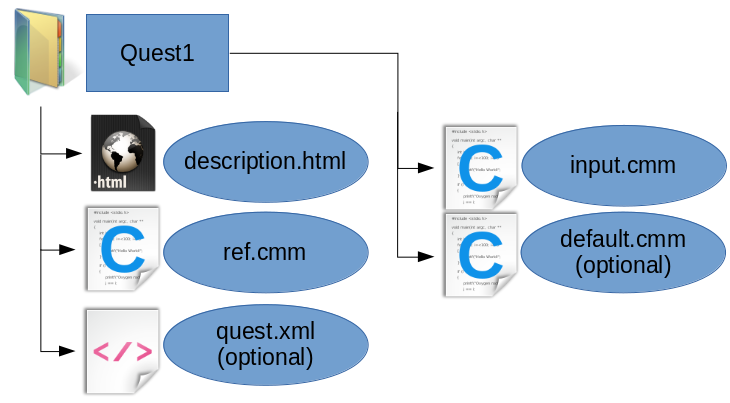
\includegraphics[width=0.8\textwidth]{./media/images/quest/quest_ordnerstruktur}
  \caption{Struktur einer Quest}
  \label{fig:struct_quest}
\end{figure}

Damit eine Quest vom Programm als solche erkannt wird, müssen mehrere Dateien vorhanden sein. Einige davon werden von der Überprüfungsroutine benötigt. Andere dienen wiederum zur Beschreibung der Quest. Dies ist in Abbildung \ref{fig:struct_quest} ersichtlich.

\begin{itemize}
\item \textbf{description.html}\\
Diese Datei beinhaltet die Beschreibung der Quest. Diese muss im \textbf{.html} Format geschrieben werden. Hier kann die Aufgabe ausführlich erklärt werden. Informationen über weiterführende Quests oder Tokens, also Auszeichnungen für fertiggestellte Quests, können auch in die Beschreibung hinzugefügt werden.

\item \textbf{ref.cmm}\\
In der \textbf{ref.cmm} befindet sich das Referenzprogramm. Dieses wird von C Compact beim Überprüfen der Quest ausgeführt. Wenn die Ausgaben des Benutzerprogramms, den Ausgaben des Referenzprogramms gleichen, wird die Aufgabe als richtig gewertet.

\item \textbf{default.cmm}\\
In der \textbf{default.cmm} befindet sich eine Quelltextvorgabe, welche beim erstmaligen Öffnen einer Quests angezeigt, beziehungsweise zur weiteren Verarbeitung zur Verfügung gestellt wird. 

Hierdurch kann die Lehrperson vorgeben, wie die Aufgabe gelöst werden kann. So könnte sich zum Beispiel in der Datei eine Reihe von Kommentaren befinden, worin der Nutzer genauere Anweisungen zur Erstellung des Programms erhält. Auch kann man dank dieser Datei Aufgaben erstellen, wo die Nutzer einen bestimmten Fehler in einem vorgegebenen Programm finden und ausbessern müssen. 

Um Fehler bei der Überprüfungsroutine zu vermeiden, können hier die Eingabe- und Ausgabefunktionen bereits definiert werden. 

\item \textbf{input.cmm}\\
Diese Datei wird zum Erstellen für Eingabedaten der \textbf{ref.cmm} verwendet. Falls man diese Datei nicht verwendet will, muss diese Datei ein leeres Programm enthalten. 
\begin{lstlisting}[language=C]
void main(){}
\end{lstlisting}
\end{itemize}

Optional können noch weitere Dateien hinzugefügt werden. Falls diese nicht funktionstüchtig sind, werden diese Dateien vom Programm ignoriert und nicht verwendet.

\begin{itemize}
\item \textbf{quest.xml}\\
In dieser Datei kann man einige Parameter der Quest definieren. Diese werden im Quest-Auswahlfenster genutzt.

\begin{lstlisting}[language=XML]
<quest>
    <title>Example-Quest-Name</title>
    <attribute>Übung</attribute>
    <token>example.xml</token>
    <matcher>REGEX</matcher>
    <previousFolder>andereQuest</previousFolder>
    <state>locked</state>
</quest>
\end{lstlisting}
Man kann einen Titel, ein Attribut, die dazugehörige Auszeichnung und einen Status bestimmen.
\begin{itemize}
\item Falls in der \textbf{quest.xml} kein Titel definiert wurde, wird automatisch der Ordnername als Titel gewählt. 
\item Sollte kein \textbf{attribute} definiert sein, bleibt dieses Feld in der Questauswahl leer.
%TODO
\item Wenn eine Quest erst dann gestartet werden soll, wenn eine andere abgeschlossen wurde, so kann dies im \textbf{previousFolder} unter Angabe des Ordnernamens der Quest definieren.
\item Bei \textbf{token}, kann man eine Auszeichnung wählen. Diese Auszeichnung ist ein Bild, Titel und eine Beschreibung, welche in der Benutzeroberfläche angezeigt wird. Sie muss im zugehörigen Package im Ordner \textbf{tokens} definiert sein. Wenn dieses nicht vorhanden oder fehlerhaft ist, wird bei Abschluss der Quest, kein Token hinzugefügt.
\item Mithilfe des \textbf{matcher} Tags, kann man eine reguläre Expressionen definieren, welche von der Überprüfungsroutine verwendet wird. Damit ist es möglich, dass das Benutzerprogramm eine leicht abgeänderte Ausgabe, als die Überprüfungsroutine, erzeugen darf. Indem man diesen Tag in verwendet, überschreibt man einen vordefinierten matcher.

\begin{lstlisting}[language=JAVA]
	public String DEFAULT_MATCHER = "([,;:\n\t])";
\end{lstlisting}
Dieser Matcher entfernt automatisch \textbf{; , :} und \textbf{Leerzeichen}.

\item Mithilfe des \textbf{Status}, kann man im vorhinein bestimmen, ob die Quest bereits abgeschlossen, gesperrt oder auswählbar ist.
\end{itemize}

\item \textbf{style.css}\\
Dieses Datei kann als Stylesheet für die dazugehörige \textbf{description.html} verwendet werden. Sie ersetzt das vordefinierte Stylesheet.

\end{itemize}

\section{Variablen in der quest.java}
\begin{lstlisting}[language=JAVA]
//Kann von der quest.xml definiert werden
	private String title;			//Titel der Quest		
	private Token token;			//Referenz zum Token
	private String matcher;			//Reguläre expression, für Auswertung benötigt
	private String state;			//locked, selectable, finished,..
	private String attribute;		//Attribut bei der Questauswahl
	private String previousFolder;	//Muss vorher eine Quest erledigt werden

//Wird durch andere Faktoren bestimmt
	private boolean description;	//Beschreibung
	private boolean style;			//extra Stylesheet
	private boolean ref;			//ref.cmm vorhanden?
	private boolean input;			//input.cmm vorhanden?	
	private boolean defaultCmm;		//default.cmm vorhanden?
	private String cmmFilePath;		//Pfad zum dazugehörigen File	
	private Date date;				//Datum der letzten Bearbeitung
	private String initPath;		//auch "packages"
	private String packagePath;		//interner Pfad des Packages
	private String questPath;		//Questordner vom Package aus

\end{lstlisting}
Wie im Kapitel \ref{sec:dateien_in_einer_quest} bereits beschrieben wurde, können hier manche Varialben in der Datei \textbf{quest.xml} definiert werden. Falls die \textbf{quest.xml} nicht vorhanden ist, werden hier Standardwerte definiert.

\begin{itemize}
\item Der Name der Quest wird anhand des Ordnernamens definiert.
\item Die Quest wird auf den Status \textbf{selectable} gesetzt, somit sind die Quests vom Benutzer immer verwendbar. Sie können somit jederzeit aus der Liste der Quests ausgewählt werden.
\item Das Attribut wird automatisch auf den String "`\textbf{exercise}"' gesetzt. Dieser wird im Quest-Package angezeigt.
\end{itemize}
%Somit wird der Titel auf den Ordnernamen gesetzt. Das Attribut wird auf exercise gesetzt und als state wird selectable gewählt, somit ist die Quest auswählbar.

Die Variablen, welche boolean als Datentyp haben, werden bei der Überprüfung der Dateien eines Questordners gesetzt. Falls die Datei vorhanden ist, wird der Wert auf true gesetzt, wenn nicht false. Das definierte Date beinhaltet die letzte Bearbeitung einer Quest und wird im Profil gespeichert.

%TODO
%Die Pfade beinhalten einen relativen Pfad. Somit enthält initPath meist packages, packagePath, den Pfad des Packages, ab "packages" und questPath den Ordnernamen der Quest. Duch diese Struktur, ist es einfach möglich, auf andere Dateien inerhalb des Packages zuzugreifen. 

%Alle hier erwähnten Variablen sind durch Getter und Setter erreichbar.


\section{Questzustände}
\label{sec:Queststate}
\begin{itemize}
\item \textbf{locked}:\\ Diese Quest kann nicht bearbeitet werden. Die Quest wird automatisch auf diesen Zustand gesetzt, falls in der \textbf{quest.xml} für \textbf{previousFolder} ein Wert gesetzt, und dieser Wert im Profil noch nicht als fertiggestellt markiert wurde. Dieser Zustand wird dazu benötigt, um Quests, welche erst nach Beendigung einer anderen Quest freigeschaltet werden, zu sperren.
\item \textbf{selectable}:\\ Der Benutzer kann diese Quest auswählen. Dies hier ist der Standardzustand.
\item \textbf{inprogress}:\\ Der Benutzer hat diese Quest bereits begonnen, jedoch noch nicht abgeschlossen. Quests, welche diese Kritierien erfüllen, werden automatisch von \textbf{open} auf diesen Status gesetzt, sobald eine neue Quest geöffnet wurde.
\item \textbf{open}:\\ Diese Quest wird gerade vom Benutzer bearbeitet. Durch diesen Tag kann im Profil die zuletzt geöffnete Quest festgestellt werden. Sobald ein Profil geöffnet wird, wird somit die zuletzt verwendete Quest geöffnet.
\item \textbf{finished}:\\ Die Quest wurde fertiggestellt und von der Überprüfungsroutine als richtig empfunden.
\end{itemize}

\section{Linearer Questweg}
In so gut wie allen Spielen, von denen sich unser Questsystem ableitet gibt es einen Hauptquestweg. Darin wird der Benutzer in die Geschichte eingeführt und erlebt Abenteuer. In unserem Fall wäre so ein Questweg für den Lernfortschritt sehr förderlich, da der Benutzer Schritt für Schritt immer komplexere und anspruchsvollere Aufgaben meistern muss.

Der Ersteller kann selbst entscheiden, ob man, bevor man eine schwierigere Quest starten kann, eine einfachere vorher abschließen muss. In unserem Fall ist der lineare Questweg sehr förderlich, da der Benutzer Schritt für Schritt immer komplexere und anspruchsvollere Aufgaben meistern muss. Somit, passt dies auch in das klassische Konzept des derzeigen Unterrichts: Aufgaben werden immer schwieriger.

Der Lineare Questweg kann mit dem Attribut \textbf{previousFolder} umgesetzt werden.